% Template visuel repris depuis TFIDF/presentation/main.tex.
% Presentation: BERT et explicabilite des modeles.
\documentclass[10pt]{beamer}
\usepackage[utf8]{inputenc}
% Le template original charge xeCJK. On le garde seulement si sa dependance
% locale est disponible, afin que la presentation compile aussi sans support CJK.
\IfFileExists{ctexhook.sty}{\usepackage{xeCJK}}{}
\usepackage{graphicx}
\IfFileExists{mathtools.sty}{\usepackage{mathtools}}{}
\IfFileExists{utopia.sty}{\usepackage{utopia}}{}
\usetheme{CambridgeUS}
\usecolortheme{dolphin}
\usepackage{tcolorbox}
\IfFileExists{tabularray.sty}{\usepackage{tabularray}}{}
\IfFileExists{float.sty}{\usepackage{float}}{}
\IfFileExists{adjustbox.sty}{\usepackage{adjustbox}}{}
\IfFileExists{caption.sty}{\usepackage{caption}}{}
\IfFileExists{subcaption.sty}{\usepackage{subcaption}}{}
\IfFileExists{multirow.sty}{\usepackage{multirow}}{}
\usepackage{tikz}
\IfFileExists{booktabs.sty}{\usepackage{booktabs}}{%
    \newcommand{\toprule}{\hline}
    \newcommand{\midrule}{\hline}
    \newcommand{\bottomrule}{\hline}
}
\IfFileExists{makecell.sty}{\usepackage{makecell}}{}
\usepackage{array}
\usepackage{longtable}
\IfFileExists{natbib.sty}{\usepackage{natbib}}{}
\usepackage{hyperref}
\providecommand\theadfont{}
\renewcommand\theadfont{\bfseries}

\usetikzlibrary{positioning}
\usetikzlibrary{calc}
\usetikzlibrary{arrows.meta}
\usetikzlibrary{shapes}
\usetikzlibrary{shapes.geometric}

% Palette conservee depuis le template original.
\definecolor{lightred}{RGB}{180,227,236}
\definecolor{middlelightred}{RGB}{138,22,57}
\definecolor{middledered}{RGB}{217,79,120}
\definecolor{redforsnnu}{RGB}{176,44,89}
\definecolor{darkred}{RGB}{138,22,57}

\setbeamercolor*{palette primary}{bg=redforsnnu, fg=white}
\setbeamercolor*{palette secondary}{bg=middledered, fg=white}
\setbeamercolor*{palette tertiary}{bg=middlelightred, fg=white}
\setbeamercolor*{titlelike}{fg=redforsnnu}
\setbeamercolor*{title}{bg=darkred, fg=white}
\setbeamercolor*{item}{fg=redforsnnu}
\setbeamercolor*{caption name}{fg=middledered}

\usefonttheme{professionalfonts}

% Affiche une vraie figure si elle existe, sinon un placeholder compilable.
% Remplacer progressivement les chemins par des exports propres dans figures/*.pdf.
\newcommand{\safegraphic}[2][0.85\linewidth]{%
    \IfFileExists{#2}{%
        \includegraphics[width=#1]{#2}%
    }{%
        \begin{tcolorbox}[width=#1, colback=lightred!20, colframe=redforsnnu, title=Figure a completer]
            \centering
            \scriptsize
            Placeholder pour la figure attendue.\\[0.15cm]
            {\tiny\url{#2}}
        \end{tcolorbox}%
    }%
}

\newcommand{\safegraphicfit}[3][0.85\linewidth]{%
    \IfFileExists{#3}{%
        \includegraphics[width=#1,height=#2,keepaspectratio]{#3}%
    }{%
        \begin{tcolorbox}[width=#1, colback=lightred!20, colframe=redforsnnu, title=Figure a completer]
            \centering
            \scriptsize
            Placeholder pour la figure attendue.\\[0.15cm]
            {\tiny\url{#3}}
        \end{tcolorbox}%
    }%
}

\newcommand{\highlight}[1]{\textcolor{redforsnnu}{\textbf{#1}}}

\titlegraphic{
\begin{tikzpicture}[overlay, remember picture]
    \node[anchor=north, yshift=-0.7cm] at (current page.north){
        \begin{minipage}{\textwidth}
            \centering
            \IfFileExists{images/logo.png}{%
                
\includegraphics[height=1.7cm]{images/logo.png}%
            }{%
                \IfFileExists{images/logo.jpg}{%
                    
\includegraphics[height=1.7cm]{images/logo.jpg}%
                }{%
                    \vspace{0.2cm}
                    {\small Universite Paris Cite}
                }%
            }
        \end{minipage}
    };
\end{tikzpicture}
}

\setbeamerfont{title}{size=\large}
\setbeamerfont{subtitle}{size=\small}
\setbeamerfont{author}{size=\small}
\setbeamerfont{date}{size=\small}
\setbeamerfont{institute}{size=\scriptsize}

\title[]{Explicabilité des modèles de classification de textes,\\ application NLP -- Approche BERT}
\subtitle{}
\author[]{\textbf{Sofiane AGOUNI KACI}}
\institute[]{Modélisation des systèmes intelligents\\Master 2 vision et machine intelligente}
\date[\textcolor{white}{2026}]{2026}

\AtBeginSection[]{
  \begin{frame}
  \vfill
  \transfade
  \centering
  \begin{beamercolorbox}[sep=8pt,center,shadow=true,rounded=true]{title}
    \usebeamerfont{title}\insertsectionhead\par%
  \end{beamercolorbox}
  \vfill
  \end{frame}
}

\begin{document}

\begin{frame}[plain]
    \inserttitlegraphic
    \vspace*{2.35cm}
    \begin{center}
        \begin{beamercolorbox}[sep=8pt,center,shadow=true,rounded=true]{title}
            \usebeamerfont{title}\inserttitle\par
        \end{beamercolorbox}
        \vspace{0.45cm}
        {\usebeamerfont{author}\insertauthor\par}
        \vspace{0.25cm}
        {\usebeamerfont{institute}\insertinstitute\par}
        \vspace{0.35cm}
        {\usebeamerfont{date}\insertdate\par}
    \end{center}
\end{frame}

\begin{frame}{Table of Contents}
    \tableofcontents
\end{frame}

%------------------------------------------------------------
\section{Contexte}
%------------------------------------------------------------

\begin{frame}{Probleme et objectif}
    \vspace{-0.15cm}
    \begin{itemize}\scriptsize
        \item Comparer le fine-tuning complet de BERT et le linear probing.
        \item Expliquer les decisions du modele avec SHAP, LIME et les poids d'attention.
    \end{itemize}
    \vspace{0.02cm}
    \centering
    \safegraphicfit[0.97\linewidth]{0.66\textheight}{images/overview.png}
\end{frame}

\begin{frame}{Dataset}
    \vspace{-0.2cm}
    \begin{columns}[T,onlytextwidth]
        \begin{column}{0.40\textwidth}
            \begin{tcolorbox}[colback=lightred!20, colframe=redforsnnu, title=Taille des splits]
                \tiny
                \begin{center}
                \setlength{\tabcolsep}{2pt}
                \begin{tabular}{@{}lrrr@{}}
                    \toprule
                    Split & Total & Femme & Homme \\
                    \midrule
                    Train & 852 & 492 & 360 \\
                    Val. & 284 & 164 & 120 \\
                    Test & 285 & 165 & 120 \\
                    \bottomrule
                \end{tabular}
                \end{center}
            \end{tcolorbox}
            \begin{itemize}\small
                \item Les labels sont extraits des noms de fichiers.
                \item Les distributions sont proches entre validation et test.
                \item Risque: biais possibles dans les donnees et dans le protocole de labellisation.
            \end{itemize}
        \end{column}
        \begin{column}{0.52\textwidth}
            \centering
            \vspace{-0.12cm}
            \begin{minipage}{\linewidth}
                \centering
                \safegraphicfit[0.78\linewidth]{0.24\textheight}{images/distribution_total.png}\\[-0.02cm]
                {\tiny Distribution totale homme/femme\par}
            \end{minipage}

            \vspace{0.08cm}
            \begin{minipage}{\linewidth}
                \centering
                \safegraphicfit[0.78\linewidth]{0.24\textheight}{images/distribution_splits.png}\\[-0.02cm]
                {\tiny Distribution des classes par split\par}
            \end{minipage}
        \end{column}
    \end{columns}
\end{frame}

\begin{frame}{Pipeline global}
    \begin{figure}
    \centering
    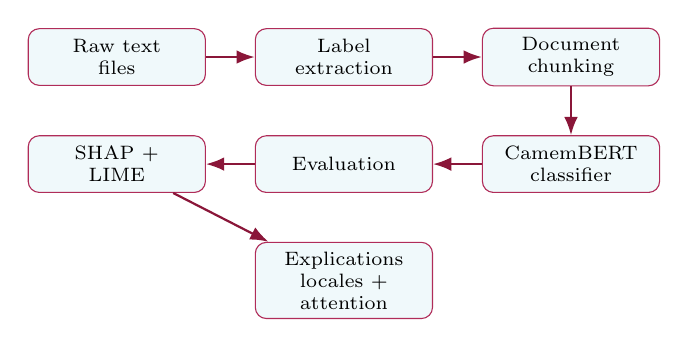
\begin{tikzpicture}[
        node distance=0.62cm,
        box/.style={draw=redforsnnu, rounded corners, fill=lightred!20,
                    minimum width=2.25cm, minimum height=0.72cm,
                    align=center, font=\scriptsize},
        arrow/.style={-Latex, thick, draw=darkred}
    ]
        \node[box] (raw) {Raw text\\files};
        \node[box, right=of raw] (labels) {Label\\extraction};
        \node[box, right=of labels] (tfidf) {Document\\chunking};
        \node[box, below=of tfidf] (mlp) {CamemBERT\\classifier};
        \node[box, left=of mlp] (eval) {Evaluation};
        \node[box, left=of eval] (xai) {SHAP +\\LIME};
        \node[box, below=of eval] (pert) {Explications\\locales +\\attention};

        \draw[arrow] (raw) -- (labels);
        \draw[arrow] (labels) -- (tfidf);
        \draw[arrow] (tfidf) -- (mlp);
        \draw[arrow] (mlp) -- (eval);
        \draw[arrow] (eval) -- (xai);
        \draw[arrow] (xai) -- (pert);
    \end{tikzpicture}
    \end{figure}

\end{frame}

%------------------------------------------------------------
\section{Architecture du classifieur}
%------------------------------------------------------------

\begin{frame}{Decoupage des documents}
    \begin{columns}[T]
        \begin{column}{0.46\textwidth}
            \begin{tcolorbox}[colback=lightred!20, colframe=redforsnnu, title=Parametres de chunking]
                \begin{itemize}\small
                    \item 64 chunks par document pour la classe \texttt{homme}.
                    \item 32 chunks par document pour la classe \texttt{femme}.
                \end{itemize}
            \end{tcolorbox}
        \end{column}
        \begin{column}{0.48\textwidth}
            \begin{tcolorbox}[colback=middledered!20, colframe=darkred, title=Justification]
                \small
                Ce choix est utilise car il y a beaucoup plus de documents \texttt{femme}
                que de documents \texttt{homme}. Le nombre de chunks par document est ajuste
                pour limiter le desequilibre effectif pendant l'apprentissage.
            \end{tcolorbox}
        \end{column}
    \end{columns}
\end{frame}

\begin{frame}{Architecture du reseau}
    \centering
    \safegraphicfit[0.95\linewidth]{0.76\textheight}{images/architecture_reseau.png}
\end{frame}

\begin{frame}{Entrainement 1 -- fine-tuning complet de BERT}
    \begin{tcolorbox}[colback=lightred!20, colframe=redforsnnu, title=Hyperparametres]
        \scriptsize
        \begin{tabular}{@{}lll@{\hspace{0.6cm}}lll@{}}
            Taille de batch & = & 32 &
            Batch d'evaluation & = & 32 \\
            Nombre d'epoques & = & 5 &
            Taux d'apprentissage & = & \texttt{2e-5} \\
            Optimiseur & = & AdamW &
            & &
        \end{tabular}
    \end{tcolorbox}
    \vspace{0.05cm}
    \begin{columns}[T]
        \begin{column}{0.50\textwidth}
            \centering
            \safegraphicfit[0.98\linewidth]{0.48\textheight}{images/finetuning_loss.png}
            {\centering\tiny Courbes d'entrainement\par}
        \end{column}
        \begin{column}{0.48\textwidth}
            \centering
            \safegraphicfit[0.92\linewidth]{0.48\textheight}{images/matrice_confusion_finetuning.png}
            {\centering\tiny Matrice de confusion -- fine-tuning\par}
        \end{column}
    \end{columns}
\end{frame}

\begin{frame}{Entrainement 2 -- linear probing}
    \begin{tcolorbox}[colback=lightred!20, colframe=redforsnnu, title=Hyperparametres]
        \scriptsize
        \begin{tabular}{@{}lll@{\hspace{0.6cm}}lll@{}}
            Taille de batch & = & 32 &
            Batch d'evaluation & = & 32 \\
            Nombre d'epoques & = & 5 &
            Taux d'apprentissage & = & \texttt{2e-5} \\
            Optimiseur & = & AdamW &
            & &
        \end{tabular}
    \end{tcolorbox}
    \vspace{0.05cm}
    \centering
    \safegraphicfit[0.78\linewidth]{0.47\textheight}{images/linear_probing_loss.png}
\end{frame}

%------------------------------------------------------------
\section{Evaluation}
%------------------------------------------------------------

\begin{frame}{Evaluation -- linear probing}
    \begin{columns}[T,totalwidth=\textwidth]
        \column{0.47\textwidth}
            \centering
            \safegraphicfit[0.98\linewidth]{0.72\textheight}{images/confusion_matrix_linear_probing.png}

        \column{0.50\textwidth}
            \begin{tcolorbox}[colback=lightred!15, colframe=redforsnnu, title=Scores par classe]
                \centering
                \tiny
                \begin{tabular}{@{}lccc@{}}
                    \toprule
                    Classe & Precision & Recall & F1-score \\
                    \midrule
                    femme & 82.1\% & 80.6\% & 81.3\% \\
                    homme & 74.0\% & 75.8\% & 74.9\% \\
                    \midrule
                    \multicolumn{3}{l}{Accuracy globale} & 78.6\% \\
                    \bottomrule
                \end{tabular}
            \end{tcolorbox}
            \vspace{0.12cm}
            \centering
            \safegraphicfit[0.98\linewidth]{0.34\textheight}{images/roc_curve.png}
    \end{columns}
\end{frame}

%------------------------------------------------------------
\section{Explicabilite}
%------------------------------------------------------------

\begin{frame}{SHAP}
    \centering
    \vfill
    {\small\textbf{Principe de la methode SHAP}\par}
    \vspace{0.08cm}
    \makebox[\textwidth][c]{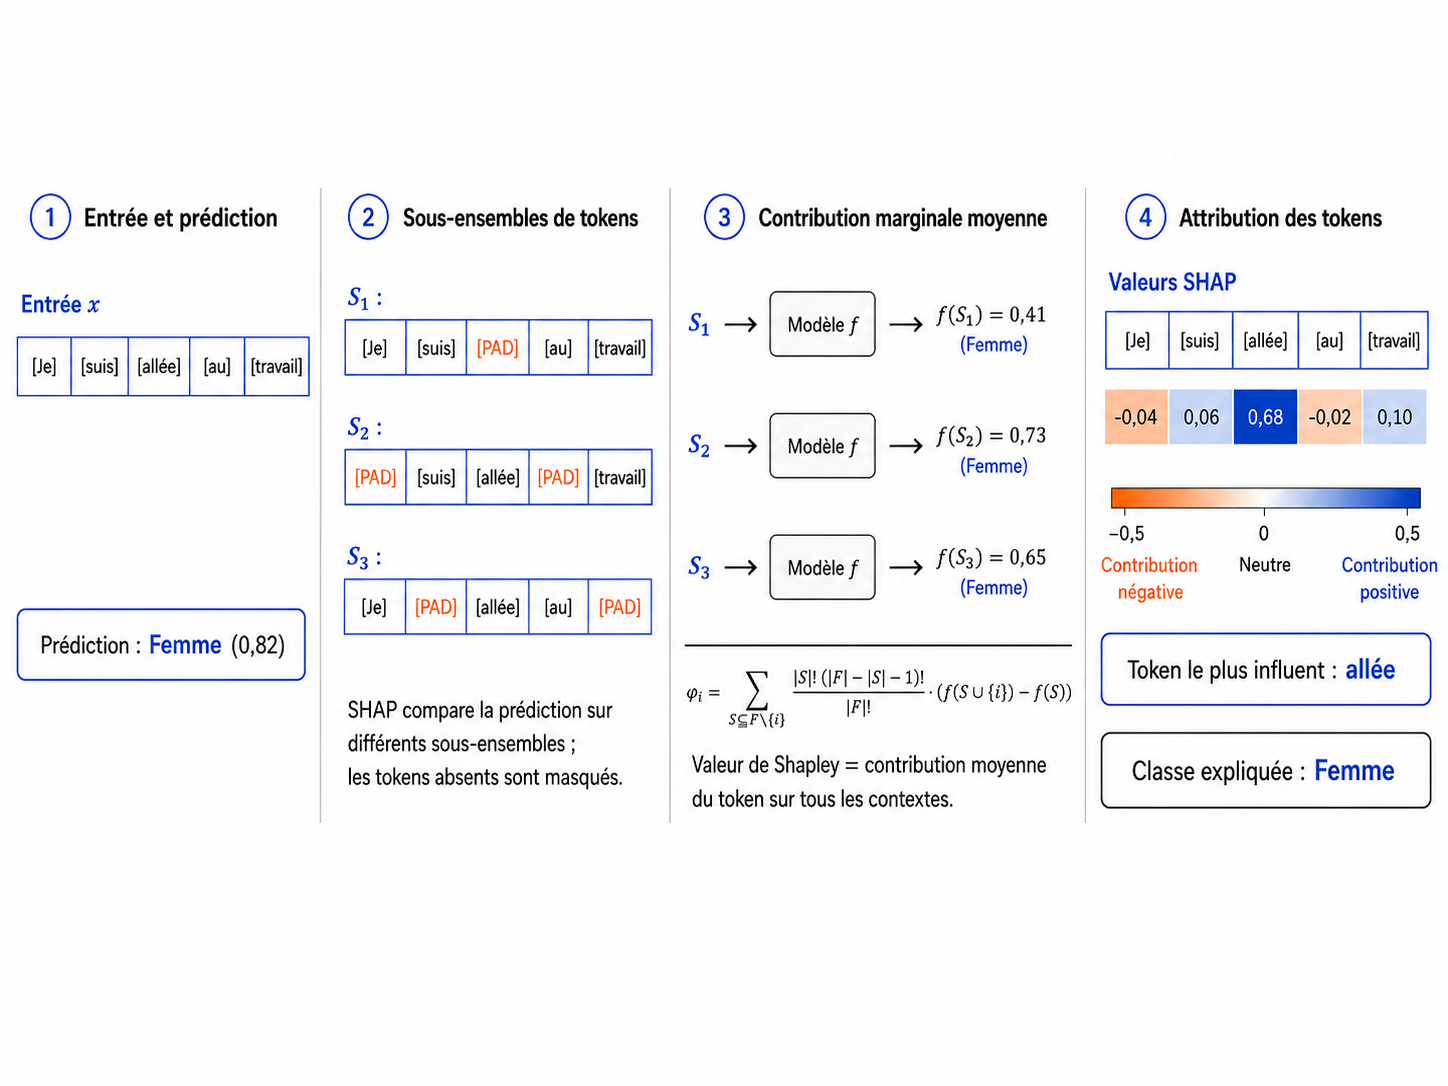
\includegraphics[width=0.88\textwidth,height=0.64\textheight,keepaspectratio]{images/SHAP.png}}
    \vspace{0.06cm}
    {\tiny Source: image generee par IA, prompt engineering.\par}
    \vfill
\end{frame}

\begin{frame}{LIME}
    \centering
    \vfill
    {\small\textbf{Principe de la methode LIME}\par}
    \vspace{0.08cm}
    \makebox[\textwidth][c]{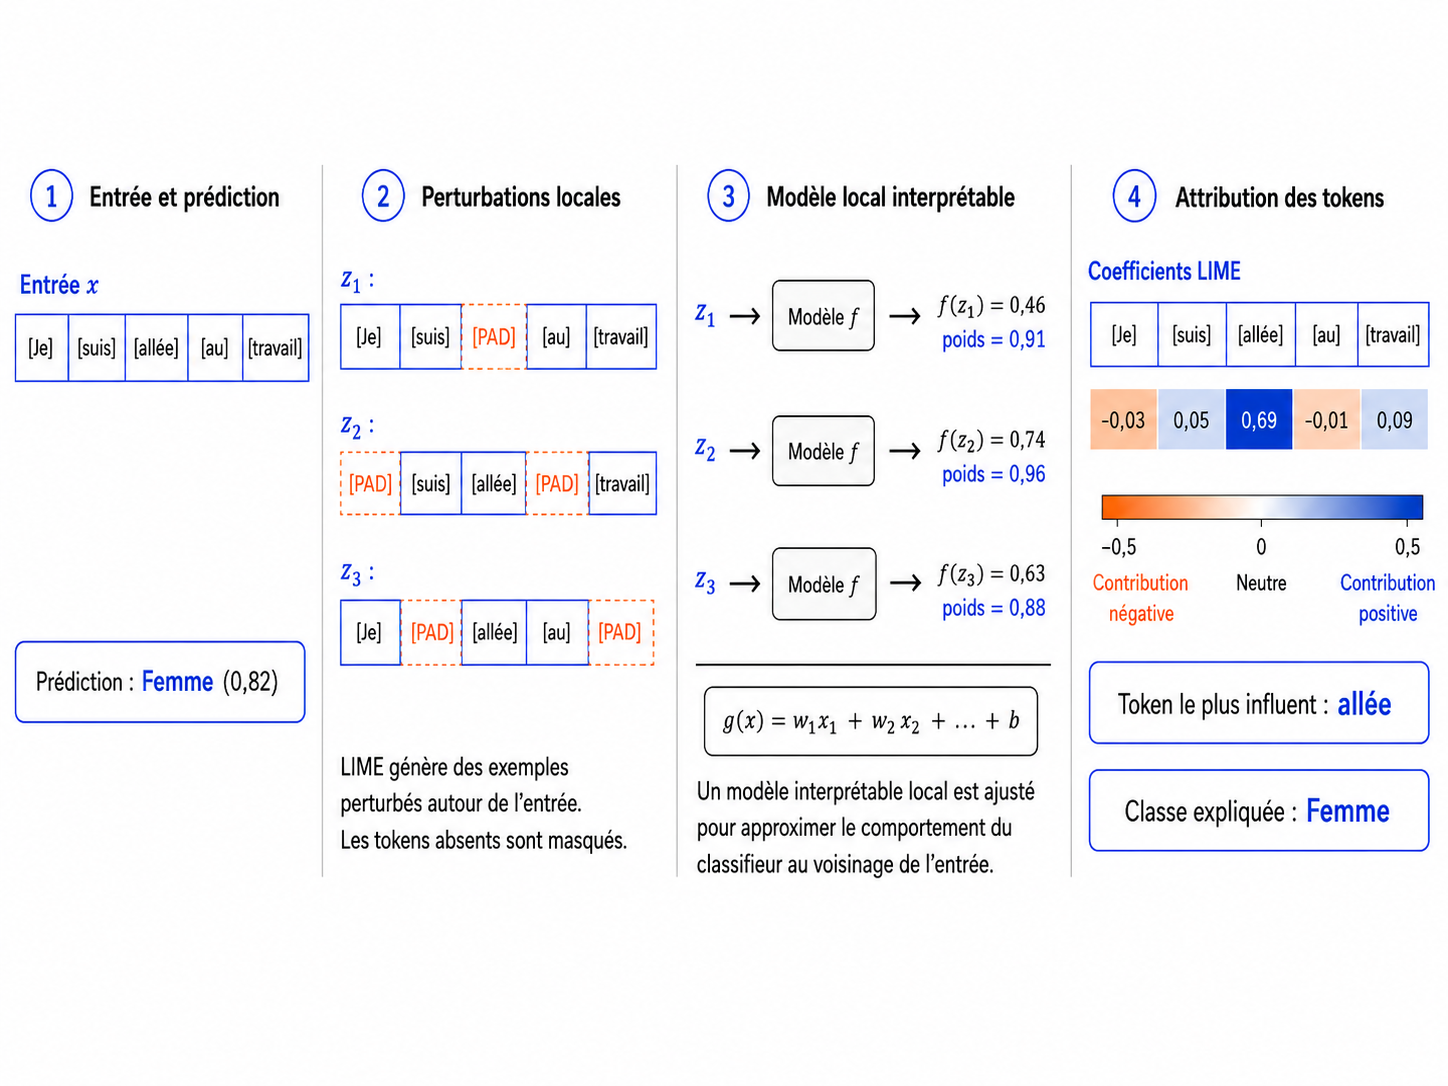
\includegraphics[width=0.88\textwidth,height=0.64\textheight,keepaspectratio]{images/LIME.png}}
    \vspace{0.06cm}
    {\tiny Source: image generee par IA, prompt engineering.\par}
    \vfill
\end{frame}

\begin{frame}{Explications globales: SHAP}
    \begin{columns}[T]
        \begin{column}{0.49\textwidth}
            \centering
            \safegraphic[0.98\linewidth]{images/shap_top_homme_terms.png}
            {\centering\scriptsize Termes soutenant les predictions \texttt{homme}\par}
        \end{column}
        \begin{column}{0.49\textwidth}
            \centering
            \safegraphic[0.98\linewidth]{images/shap_top_femme_terms.png}
            {\centering\scriptsize Termes soutenant les predictions \texttt{femme}\par}
        \end{column}
    \end{columns}
\end{frame}

\begin{frame}{Explications globales: LIME}
    \begin{columns}[T]
        \begin{column}{0.49\textwidth}
            \centering
            \safegraphic[0.98\linewidth]{images/lime_top_homme_terms.png}
            {\centering\scriptsize Termes soutenant les predictions \texttt{homme}\par}
        \end{column}
        \begin{column}{0.49\textwidth}
            \centering
            \safegraphic[0.98\linewidth]{images/lime_top_femme_terms.png}
            {\centering\scriptsize Termes soutenant les predictions \texttt{femme}\par}
        \end{column}
    \end{columns}
    \vspace{0.28cm}
    \centering
    \scriptsize LIME approxime localement le comportement du classifieur autour d'un exemple.
\end{frame}

\begin{frame}{Comparaison entre SHAP et LIME}
    \begin{columns}[T,onlytextwidth]
        \begin{column}{0.54\textwidth}
            \begin{itemize}\small
                \item Les termes communs entre SHAP et LIME indiquent les indices lexicaux les plus stables pour chaque classe.
                \item On observe une convergence partielle entre les deux methodes, ce qui renforce la confiance dans ces termes.
                \item Ces termes restent toutefois lies au dataset et ne doivent pas etre interpretes comme des regles generales.
            \end{itemize}
        \end{column}
        \begin{column}{0.42\textwidth}
            \centering
            {\small\textbf{Termes communs}\par}
            \vspace{0.18cm}
            \scriptsize
            \begin{tabular}{@{}ll@{}}
                \toprule
                Classe & Termes communs \\
                \midrule
                Homme & \textit{je, de, il, j} \\
                Femme & \textit{l, elle, les, marie, suis, d, seule} \\
                \bottomrule
            \end{tabular}
        \end{column}
    \end{columns}
\end{frame}

\begin{frame}{Explication locale: SHAP}
    \centering
    \safegraphicfit[0.92\linewidth]{0.74\textheight}{images/shap_local_explanation.png}
\end{frame}

\begin{frame}{Explication locale: LIME}
    \centering
    \safegraphicfit[0.92\linewidth]{0.74\textheight}{images/lime_local_explanation.png}
\end{frame}

\begin{frame}{Visualisation des scores d'attribution}
    \centering
    {\small\textbf{Scores d'attribution directement projetes sur le texte}\par}
    \vspace{0.12cm}
    \safegraphicfit[0.92\linewidth]{0.68\textheight}{images/text_highlight.png}
\end{frame}

\begin{frame}{Attention weights}
    \centering
    \safegraphicfit[0.92\linewidth]{0.74\textheight}{images/attention_weights.png}
\end{frame}

%------------------------------------------------------------
\section{Limites et conclusion}
%------------------------------------------------------------

\begin{frame}{Limites}
    \begin{columns}[T]
        \begin{column}{0.48\textwidth}
            \begin{tcolorbox}[colback=lightred!20, colframe=redforsnnu, title=Representation et donnees]
                \begin{itemize}\small
                    \item BERT est plus couteux a entrainer et a expliquer.
                    \item Les labels et les textes peuvent contenir des biais.
                    \item Les resultats dependent du chunking et de ce corpus.
                \end{itemize}
            \end{tcolorbox}
        \end{column}
        \begin{column}{0.48\textwidth}
            \begin{tcolorbox}[colback=middledered!20, colframe=darkred, title=Explicabilite]
                \begin{itemize}\small
                    \item Les explications SHAP/LIME sont specifiques au modele.
                    \item Les visualisations locales dependent fortement de l'exemple choisi.
                    \item Les explications locales peuvent varier selon les exemples choisis.
                \end{itemize}
            \end{tcolorbox}
        \end{column}
    \end{columns}
\end{frame}

\begin{frame}{Conclusion}
    \begin{tcolorbox}[colback=lightred!20, colframe=redforsnnu, title=Messages a retenir]
        \begin{enumerate}\small
            \item BERT/CamemBERT permet de modeliser le contexte lexical des textes.
            \item Fine-tuning complet et linear probing testent deux regimes d'apprentissage.
            \item SHAP et LIME identifient les termes qui influencent les predictions.
            \item Les explications locales et les attention weights rendent les decisions plus inspectables.
            \item On explique ce classifieur sur ce dataset, pas le langage humain en general.
        \end{enumerate}
    \end{tcolorbox}
\end{frame}

\begin{frame}[plain]
    \centering
    \vfill
    {\Large\textbf{Merci pour votre attention}\par}
    \vspace{0.8cm}
    {\Huge\textbf{Questions ?}\par}
    \vfill
\end{frame}

\end{document}
